% =========================================================
% CHAPTER 5 — TECHNOLOGY STACK
% =========================================================
\chapter{Technology Stack}

\section{Chrome Extension Framework (Manifest V3)}
The frontend is built using the Chrome Extensions API adhering to the Manifest V3 specifications. Manifest V3 represents a significant paradigm shift from V2, prioritizing user privacy, security, and performance. 
\begin{itemize}
    \item \textbf{Service Workers:} Unlike persistent background pages in V2, Manifest V3 utilizes event-driven Service Workers that terminate when idle, reducing browser memory usage.
    \item \textbf{Declarative Net Request API:} Enhances security by restricting the extension's ability to intercept arbitrary network requests, mitigating potential data leaks.
\end{itemize}

\section{JavaScript and Web APIs}
Vanilla JavaScript (ES6+) is employed for all client-side logic to ensure zero dependency bloat and maximum execution speed. 
\begin{itemize}
    \item \textbf{DOM API:} For traversing and manipulating the HTML structure.
    \item \textbf{MutationObserver API:} Critical for supporting modern Single Page Applications (React, Angular, Vue) by triggering extraction logic only when specific nodes are added or modified in the DOM tree.
    \item \textbf{Chrome Storage API:} Utilized for persisting tab-specific threat metrics, overall risk scores, and recent detections.
\end{itemize}

\section{FastAPI Backend Framework}
FastAPI is a modern, high-performance web framework for building APIs with Python 3.7+ based on standard Python type hints.
\begin{itemize}
    \item \textbf{Asynchronous Architecture:} Built on Starlette and Pydantic, FastAPI natively supports asynchronous coroutines, enabling concurrent processing of payloads from multiple active browser tabs.
    \item \textbf{Type Validation and Routing:} Pydantic schemas enforce type validation on elements, and FastAPI handles request routing and validation errors automatically.
\end{itemize}

\section{Python and Deep Learning Ecosystem}
The backend relies heavily on the Python scientific computing and cybersecurity ecosystems.
\begin{itemize}
    \item \textbf{PyTorch:} The underlying tensor computation and deep learning framework used to execute the RoBERTa models.
    \item \textbf{HuggingFace Transformers:} Used to load the pre-trained \texttt{roberta-base} tokenizer and model checkpoints.
    \item \textbf{urllib.parse:} Python's standard library utilized to extract and normalize domain hostnames from raw web URLs.
    \item \textbf{re (Regular Expressions):} Employed to run high-speed heuristic scans for urgency phrases and URL domain structures.
\end{itemize}

\section{RoBERTa Transformer Model}
RoBERTa (Robustly Optimized BERT Pretraining Approach) was selected over standard BERT due to its superior performance on natural language understanding benchmarks. RoBERTa modifies BERT's pretraining procedure by removing the Next Sentence Prediction (NSP) objective and training with dynamic masking on substantially larger datasets. This allows the model to better capture the subtle semantic nuances and coercive language structures inherent in dark patterns and social engineering attempts.

% =========================================================
% CHAPTER 6 — IMPLEMENTATION DETAILS
% =========================================================
\chapter{Implementation Details}

This chapter details the engineering intricacies of the ``DESIGN TO DECEIVE'' framework, covering the extension's internal mechanisms, the backend architecture, and the hybrid detection algorithms.

\section{Frontend and Extension Design}
The extension is designed to be lightweight, ensuring that the user's browsing experience is not degraded by high CPU utilization or rendering bottlenecks.

\subsection{DOM Scanning Architecture}
The core of the client-side logic is the DOM scanner within the content script. Upon page load, the script executes a \texttt{document.querySelectorAll} targeting a predefined set of high-risk elements: \texttt{<a>}, \texttt{<button>}, \texttt{<input type="submit">}, \texttt{<form>}, and generalized \texttt{<div>} or \texttt{<span>} elements that possess specific class names typical of modal dialogs or banners.

To handle dynamic content, a \texttt{MutationObserver} is instantiated. The observer is configured to watch for \texttt{childList} and \texttt{subtree} modifications. When new nodes are injected into the DOM (e.g., an infinite scroll loading more products, or a sudden popup modal), the observer triggers the extraction function exclusively on the newly added nodes, avoiding redundant processing of the entire document.

\subsection{Batch Processing and Message Passing}
To prevent overwhelming the background service worker and the backend server with thousands of individual HTTP requests, a batching strategy is implemented. As the DOM scanner extracts text, the strings are stored in a local JavaScript array. A debounce mechanism (typically 500ms) is applied. Once the DOM stabilizes, the array is packaged into a JSON object alongside the webpage URL and a generated UUID for each element.

This payload is transmitted to the Service Worker using \texttt{chrome.runtime.sendMessage}. The Service Worker acts as the communication bridge, overcoming CORS (Cross-Origin Resource Sharing) restrictions that would otherwise block the content script from making direct requests to the FastAPI server.

\subsection{Visual Highlighting and Tooltip Rendering}
Upon receiving the threat intelligence from the backend, the content script maps the results back to the original DOM nodes using the generated UUIDs. For elements flagged as malicious, the script performs a non-destructive DOM modification. It appends a specialized CSS class (e.g., \texttt{sentinel-phishing} or \texttt{sentinel-dark-pattern}) to the element.

To prevent alert fatigue and visual clutter, the extension implements the following visual threshold rules:
\begin{itemize}
    \item \textbf{Phishing Highlights:} Only elements flagged with \texttt{phishing_risk_level === 'High Risk'} are visually outlined with a pulsating red border.
    \item \textbf{Medium and Low Risk:} These elements are logged in the popup but do not alter the webpage layout.
    \item \textbf{Tooltips:} Active event listeners (\texttt{mouseenter} and \texttt{mouseleave}) are only attached to highlighted elements, displaying their risk band, confidence score, and descriptive explanations.
\end{itemize}

\subsection{Popup Cybersecurity Dashboard}
The extension's popup interface, accessible via the browser toolbar, serves as the central command center. Built with a modern glassmorphism aesthetic and neon cybersecurity accents, the dashboard visualizes the data stored in \texttt{chrome.storage.local}.

The dashboard features:
\begin{itemize}
    \item \textbf{Global Risk Score:} A computed metric indicating the overall threat level of the current webpage, derived from the frequency and severity of detected anomalies.
    \item \textbf{Threat Counters:} Real-time statistics showing the number of phishing links and dark patterns neutralized during the session.
    \item \textbf{Detection Log:} A scrollable list detailing the exact text snippets that were flagged, along with their timestamps and categories.
\end{itemize}

\section{Backend Design and Architecture}
The backend is engineered for high throughput and low latency, utilizing FastAPI and asynchronous programming paradigms.

\subsection{FastAPI REST API Architecture}
The backend exposes a RESTful endpoint, typically \texttt{/analyze}, which accepts \texttt{POST} requests containing the batched text payloads. The endpoint is defined using FastAPI's asynchronous routing capabilities.

Pydantic models are used to define the strict schema for incoming requests and outgoing responses. This ensures robust data validation and automatic error handling if the extension sends malformed payloads.

\begin{verbatim}
class AnalyzeRequest(BaseModel):
    elements: List[DOMElement]

class PredictionResult(BaseModel):
    id: str
    is_dark_pattern: bool
    dark_pattern_class: int
    dark_pattern_conf: float
    is_phishing: bool
    phishing_conf: float
    phishing_risk_level: str
    explanation: str
    category: str
\end{verbatim}

\subsection{Backend API Validation and Functional Testing}

The FastAPI backend server was validated using the integrated Swagger/OpenAPI testing interface. The \texttt{/analyze} endpoint was tested using manually supplied DOM elements containing phishing indicators, dark pattern content, and benign navigation text.

The API validation process verified:
\begin{itemize}
    \item Correct parsing of JSON request bodies.
    \item Successful processing of webpage DOM elements.
    \item Real-time phishing and dark pattern classification.
    \item Proper risk-level assignment and confidence scoring.
    \item Accurate JSON response generation for browser-extension integration.
\end{itemize}

Figure~\ref{fig:swagger-interface} illustrates the Swagger/OpenAPI interface used for backend validation and testing.

\begin{figure}[H]
\centering
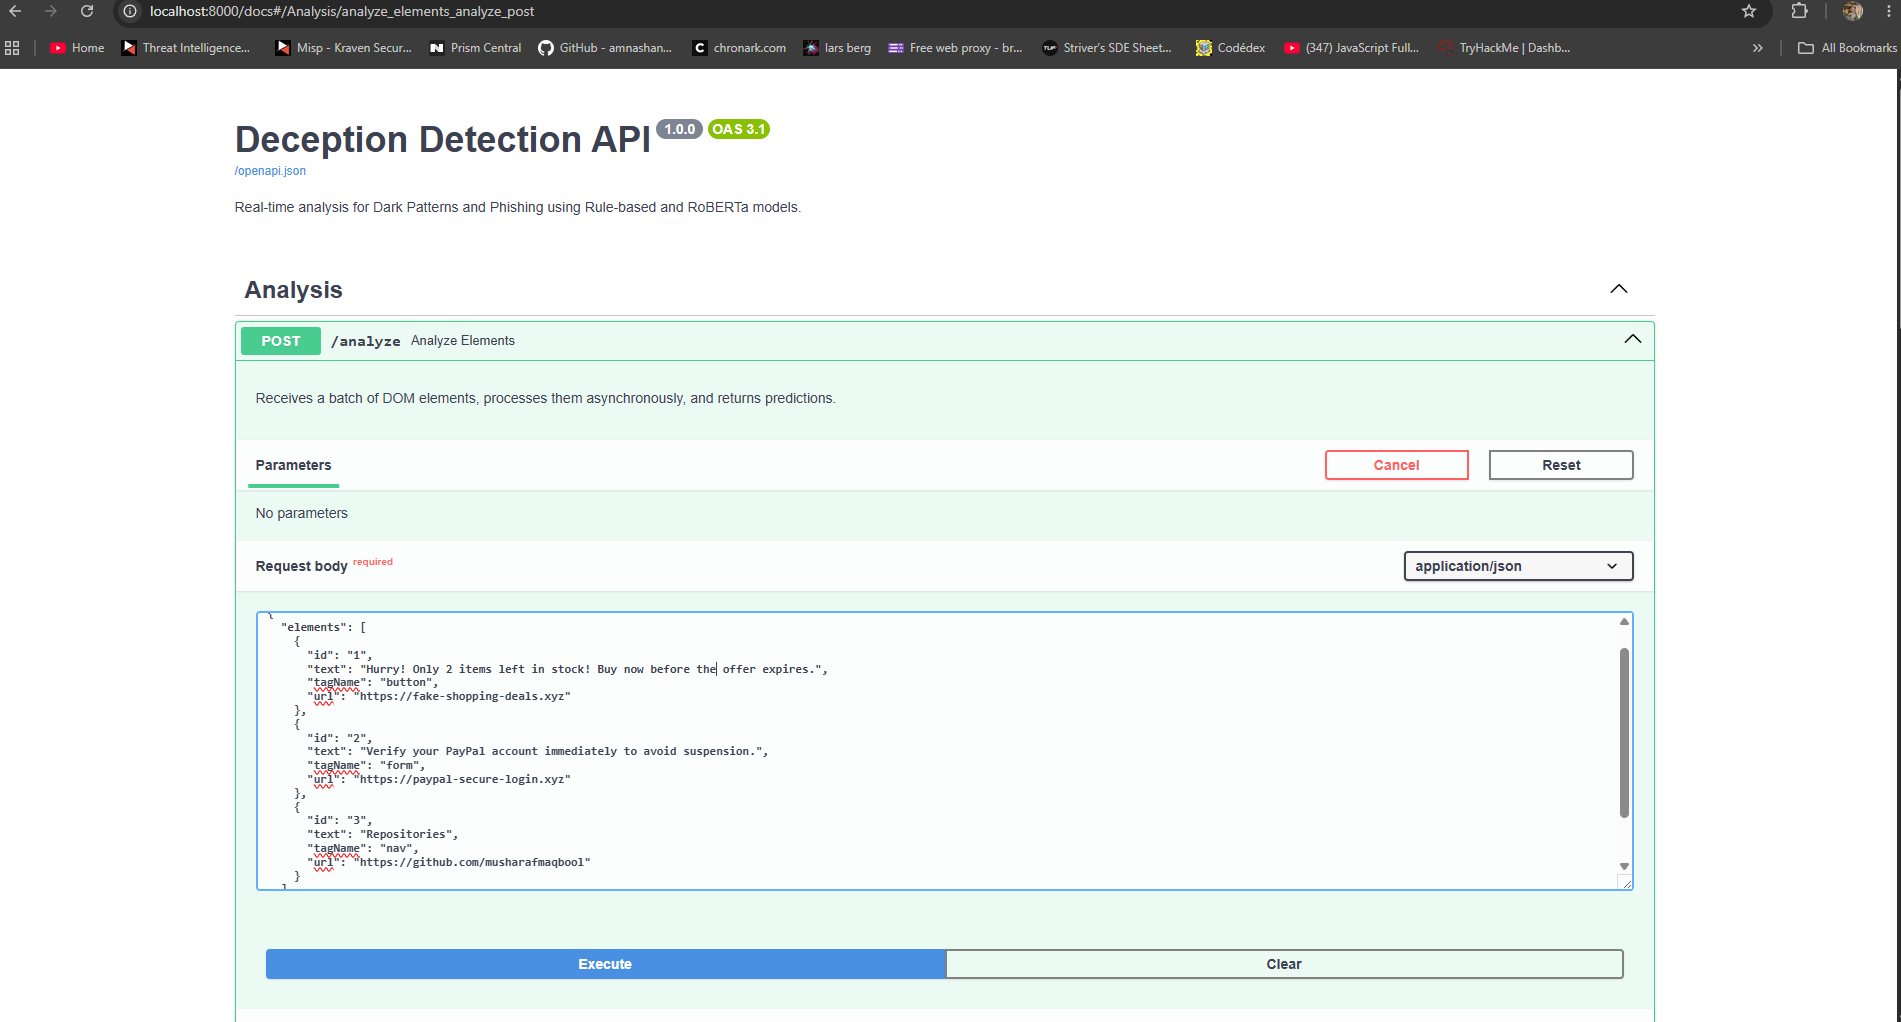
\includegraphics[width=0.92\textwidth]{Screenshot 2026-06-13 022241.png}
\caption{Swagger/OpenAPI interface for testing the FastAPI detection backend.}
\label{fig:swagger-interface}
\end{figure}

Figure~\ref{fig:api-testing} shows the testing of the \texttt{/analyze} endpoint using sample phishing and dark pattern payloads submitted in JSON format.

\begin{figure}[H]
\centering
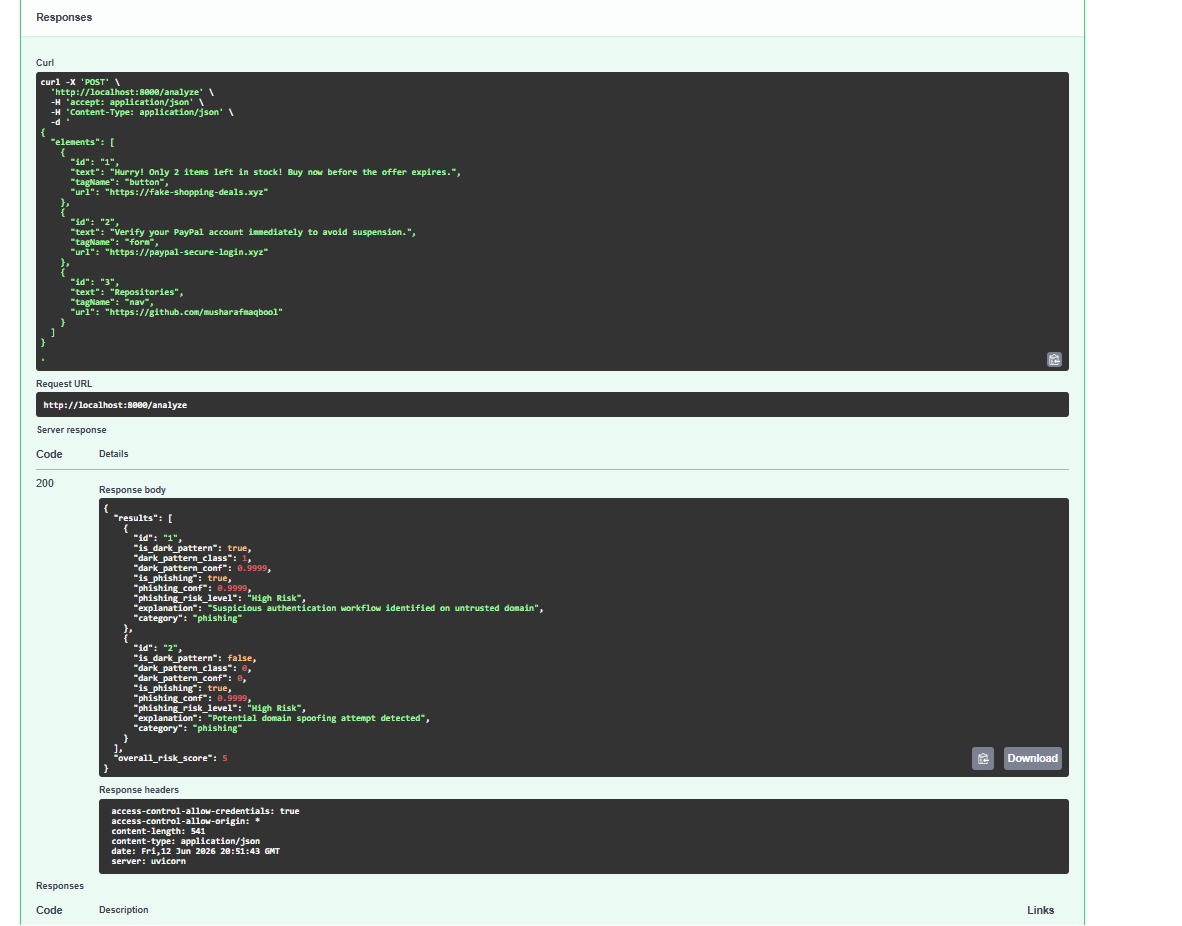
\includegraphics[width=0.92\textwidth]{Screenshot 2026-06-13 022303.png}
\caption{Execution of the \texttt{/analyze} endpoint using sample DOM elements and malicious interface text.}
\label{fig:api-testing}
\end{figure}

Figure~\ref{fig:api-response} presents the successful API response returned by the backend after inference, including phishing classification, dark pattern detection, confidence scores, explanations, and overall webpage risk scoring.

\begin{figure}[H]
\centering
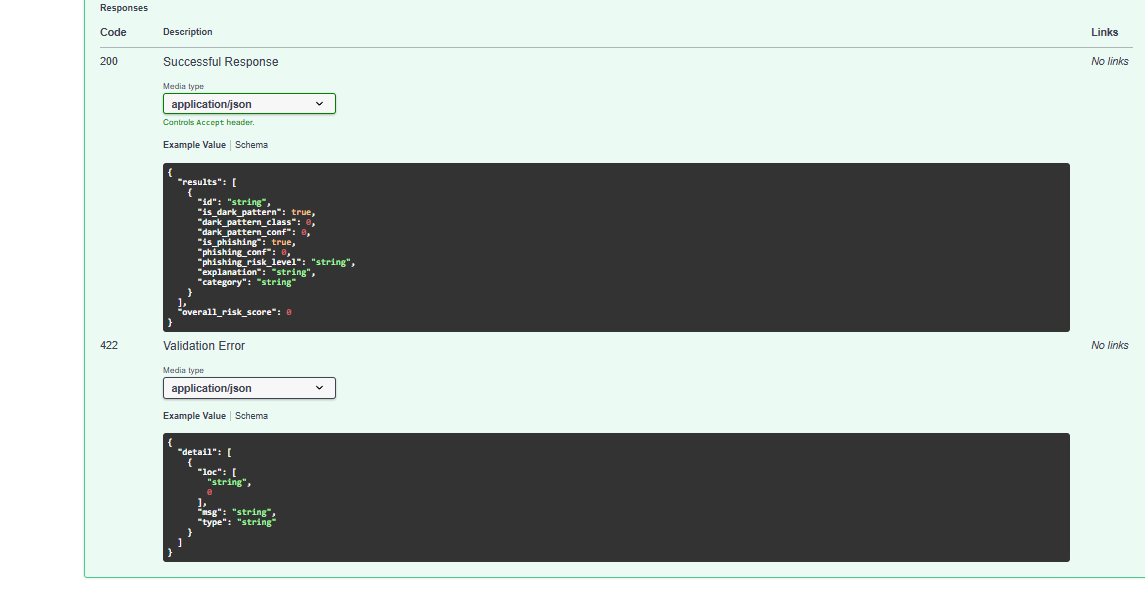
\includegraphics[width=0.92\textwidth]{Screenshot 2026-06-13 022318.png}
\caption{Successful JSON response generated by the detection backend after real-time inference.}
\label{fig:api-response}
\end{figure}

The experimental validation confirms that the proposed backend architecture can successfully analyze webpage elements dynamically and provide accurate real-time predictions for phishing and dark pattern detection within the Sentinel browser extension framework.

\subsection{Asynchronous Processing and Inference Pipeline}
When a request is received, the processing is offloaded to the \texttt{InferenceService} class. To maximize hardware utilization, the inference service loads the RoBERTa models into memory only once during application startup, utilizing FastAPI's lifecycle events.

The inference logic processes the batch of texts. The tokenizer converts the texts into uniform tensor matrices, which are then passed through the models within a thread pool executor to prevent blocking the main ASGI event loop.

\section{NLP Model Integration and Detection Algorithms}

\subsection{Trusted Domain Whitelisting and Sensitivity Tuning}
To solve the false-positive problem on legitimate services, a whitelisting system is integrated. The system maintains a compiled set of verified domains:
\begin{verbatim}
self.TRUSTED_DOMAINS = {
    "google.com", "github.com", "paypal.com", "amazon.com",
    "microsoft.com", "linkedin.com", "openai.com", "apple.com"
}
\end{verbatim}
For any element, the system extracts the domain hostname. If the domain is a trusted match (e.g. `accounts.google.com` matching `google.com` or ending with `.google.com`), the classification pipeline adjusts its parameters:
\begin{itemize}
    \item \textbf{Phishing Threshold Elevation:} The model's classification threshold for phishing is raised to a strict `0.999`.
    \item \textbf{Phishing Bypass Rule:} If the text contains standard credentials keywords but lacks urgency phrases, the ML model scan is bypassed completely, returning a safe classification.
    \item \textbf{Dark Pattern Domain Awareness:} Standard interface keywords on whitelisted platforms are automatically matched against safe-navigation classes to prevent styling blocks from being flagged as malicious.
\end{itemize}

\subsection{Dark Pattern Preprocessing and Heuristic Gating}
To eliminate false-positive detections on benign navigation panels, social metrics, and standard dashboard components without whitelisting entire domains (which would weaken academic realism), a multi-layer client-server heuristic gating pipeline is implemented:
\begin{itemize}
    \item \textbf{Short Text Length Filter:} Elements containing text shorter than 4 characters are bypassed, as they lack sufficient semantic context for linguistic manipulation analysis.
    \item \textbf{Safe UI Keyword Verification:} A compiled hash set containing standard navigation labels (e.g., \texttt{"followers"}, \texttt{"following"}, \texttt{"repositories"}, \texttt{"stars"}, \texttt{"settings"}) is evaluated against the element text. If an exact match is found, model inference is bypassed.
    \item \textbf{Structural Tag Exclusion:} The DOM parser extracts the element's parent container HTML tag. If the tag is structural navigation (\texttt{<nav>}, \texttt{<header>}, \texttt{<footer>}, \texttt{<menu>}, or \texttt{<aside>}), inference is skipped, and it is marked as safe.
    \item \textbf{Counter and Metric Regex Filter:} To capture dynamic social and profile counters (e.g., "12 Repositories", "1.2k followers", "35 stars"), the text is evaluated against a regular expression pattern:
    \begin{verbatim}
    ^\s*[\d,.]+[km]?\s*(followers|following|stars|forks|repositories|
    contributions|commits|views|members|watchers|projects|packages|
    issues|pull requests|actions|discussions)?\s*$
    \end{verbatim}
    If matched, it is bypassed as a standard UI metric.
    \item \textbf{Context-Aware Preprocessing Gate:} The heavy RoBERTa dark pattern model is executed if and only if the text contains one or more precompiled manipulative indicators (e.g., \texttt{"hurry"}, \texttt{"only"}, \texttt{"limited"}, \texttt{"last chance"}, \texttt{"no thanks"}, \texttt{"hate saving money"}). If no indicator is present, the scan is safely bypassed.
\end{itemize}

\subsection{URL Reputation Heuristic Scanning}
For untrusted domains, the system runs heuristic checks to catch common deceptive domain structures:
\begin{itemize}
    \item \textbf{Suspicious TLDs:} Evaluates if the domain ends in high-risk TLDs like `.xyz`, `.ru`, `.cc`, `.club`, or `.top`.
    \item \textbf{Excessive Hyphens:} Checks if the domain contains two or more hyphens (e.g., `verify-paypal-login`).
    \item \textbf{IP Addresses:} Verifies if the host is a raw IP address (e.g. `192.168.1.1`).
    \item \textbf{Brand Spoofing:} Splits the domain by dots and hyphens. If a trusted brand name (like `paypal` or `microsoft`) is a substring of any token on an untrusted domain (e.g., `paypal-update`), it is flagged as spoofed.
\end{itemize}

\subsection{Hybrid Classification Rule Engine}
The threat classification combines ML prediction logits with heuristic indicators:
\begin{itemize}
    \item \textbf{Rule A (Brand Spoofing):} If brand spoofing is detected, and the ML model yields confidence $\ge 0.80$, classify as High Risk phishing.
    \item \textbf{Rule B (Suspicious Domain + Heuristics):} If the domain is suspicious (TLD, hyphens, or IP), and ML confidence is $\ge 0.85$ with either urgency or credential text, classify as High Risk.
    \item \textbf{Rule C (Urgency + Credentials Combo):} If the text contains both urgency language and credential requests, and ML confidence is $\ge 0.88$, classify as High Risk.
    \item \textbf{Rule D (Direct ML Match):} If ML confidence is $\ge 0.95$ on an untrusted domain, classify as High Risk.
    \item \textbf{Rule E (Medium Risk Log):} If ML confidence is $\ge 0.80$ without supporting heuristics, classify as Medium Risk (logged but not visually highlighted).
    \item \textbf{Rule F (Low Risk):} If ML confidence is $\ge 0.50$, classify as Low Risk.
    \item \textbf{Rule G (Dark Pattern Inference):} If the text passes all dark pattern heuristic gates, the RoBERTa model is evaluated. The element is flagged as a Dark Pattern if the model predicts class 1 and its confidence is $\ge 0.995$ (our elevated threshold for visual highlighting).
\end{itemize}

\subsection{Multi-Tier Risk Bands and Score Calculation}
The webpage's overall Risk Score is calculated dynamically based on the risk levels of the flagged elements. Dark patterns carry a weight of $1.0$, High Risk phishing carries a weight of $2.0$, Medium Risk phishing carries $0.8$, and Low Risk carries $0.2$. The overall risk score $R$ is formulated as:

\begin{equation}
R = \min\left(10.0, \sum_{i=1}^{N_{dp}} (C_{dpi} \times 1.0) + \sum_{j=1}^{N_{phish}} W_{risk}(j) \times C_{phish,j} \right)
\end{equation}

Where $C$ represents the model confidence, $N$ represents the count of detections, and $W_{risk}$ is the risk tier weight. The score is capped at $10.0$ to provide a clean display in the popup dashboard.
